% Project AETHER research poster (A0 landscape). Build: tectonic AETHER_Poster.tex
\documentclass[20pt, a0paper, landscape, margin=0mm, innermargin=14mm, blockverticalspace=10mm, colspace=12mm, subcolspace=8mm]{tikzposter}
\usepackage[utf8]{inputenc}
\usepackage[T1]{fontenc}
\usepackage{lmodern}
\usepackage{amsmath, amssymb}
\usepackage{graphicx}
\usepackage{booktabs}
\usepackage{enumitem}
\setlist{nosep, leftmargin=1.2em}
\graphicspath{{../../results/figures/}{../../results/figures/fields/}{../}}

\definecolor{aetherblue}{RGB}{21,60,110}
\definecolor{aetherorange}{RGB}{214,98,20}
\definecolor{aethergrey}{RGB}{245,245,247}
\definecolorstyle{AetherStyle}{
  \colorlet{colorOne}{aetherblue}
  \colorlet{colorTwo}{aetherorange}
  \colorlet{colorThree}{aethergrey}
}{
  \colorlet{backgroundcolor}{white}
  \colorlet{framecolor}{white}
  \colorlet{titlefgcolor}{white}
  \colorlet{titlebgcolor}{colorOne}
  \colorlet{blocktitlebgcolor}{colorOne}
  \colorlet{blocktitlefgcolor}{white}
  \colorlet{blockbodybgcolor}{colorThree}
  \colorlet{blockbodyfgcolor}{black}
  \colorlet{innerblocktitlebgcolor}{colorTwo}
  \colorlet{innerblocktitlefgcolor}{white}
  \colorlet{innerblockbodybgcolor}{white}
  \colorlet{innerblockbodyfgcolor}{black}
  \colorlet{notefgcolor}{black}
  \colorlet{notebgcolor}{white}
  \colorlet{noteframecolor}{colorTwo}
}
\usetheme{Default}
\usecolorstyle{AetherStyle}
\useblockstyle{Basic}
\tikzposterlatexaffectionproofoff
\usetitlestyle{Filled}

\title{\parbox{0.95\linewidth}{\centering Project AETHER: which capsule shape slows you down without burning you up?}}
\author{Adithya Kesan Jayakanth \quad\textbar\quad adithya.kesan@icloud.com}
\institute{A multi-objective shape study of an Apollo-like re-entry capsule heat shield, June--August 2026}

\begin{document}
\maketitle[width=0.98\textwidth]

\begin{columns}

%%%%%%%%%%%%%%%%%%%%%%%%%%%%%%%%%%%%%%%%%%%%%%%%%%%%%%%%%%%%%%%% column 1
\column{0.24}

\block{1 \, The question I started from}{
A capsule needs \textbf{drag} to slow down, and the blunt face that makes the drag is where the gas is hottest. A flatter nose adds drag and spreads the heating; a sharper shoulder adds drag too, but the flow whips around the corner where the boundary layer is thinnest. Do the two goals always pull against each other, and by how much?

\vspace{4mm}
\innerblock{Bounded version of the question}{
How do the \textbf{nose radius} $R_n/D$, the \textbf{shoulder radius} $R_s/D$ and the \textbf{rear-body cone angle} $\theta_c$ of an axisymmetric Apollo-like capsule change its drag coefficient $C_D$ and the \textbf{peak heat flux} on the heat shield, at one fixed hypersonic condition?
}
\vspace{4mm}
\begin{itemize}
  \item Condition: the clean Apollo wind-tunnel test of NASA TM X-1243 (Mach 10.18, $Re_D = 1.1\times10^6$, cold wall), so there is real data to be judged against.
  \item Objectives: maximise $C_D$; minimise $q''_{\max}$ on nose cap and shoulder. Out of scope: ablation, trajectory, chemistry.
\end{itemize}
}

\block{2 \, Designing the study}{
\begin{center}
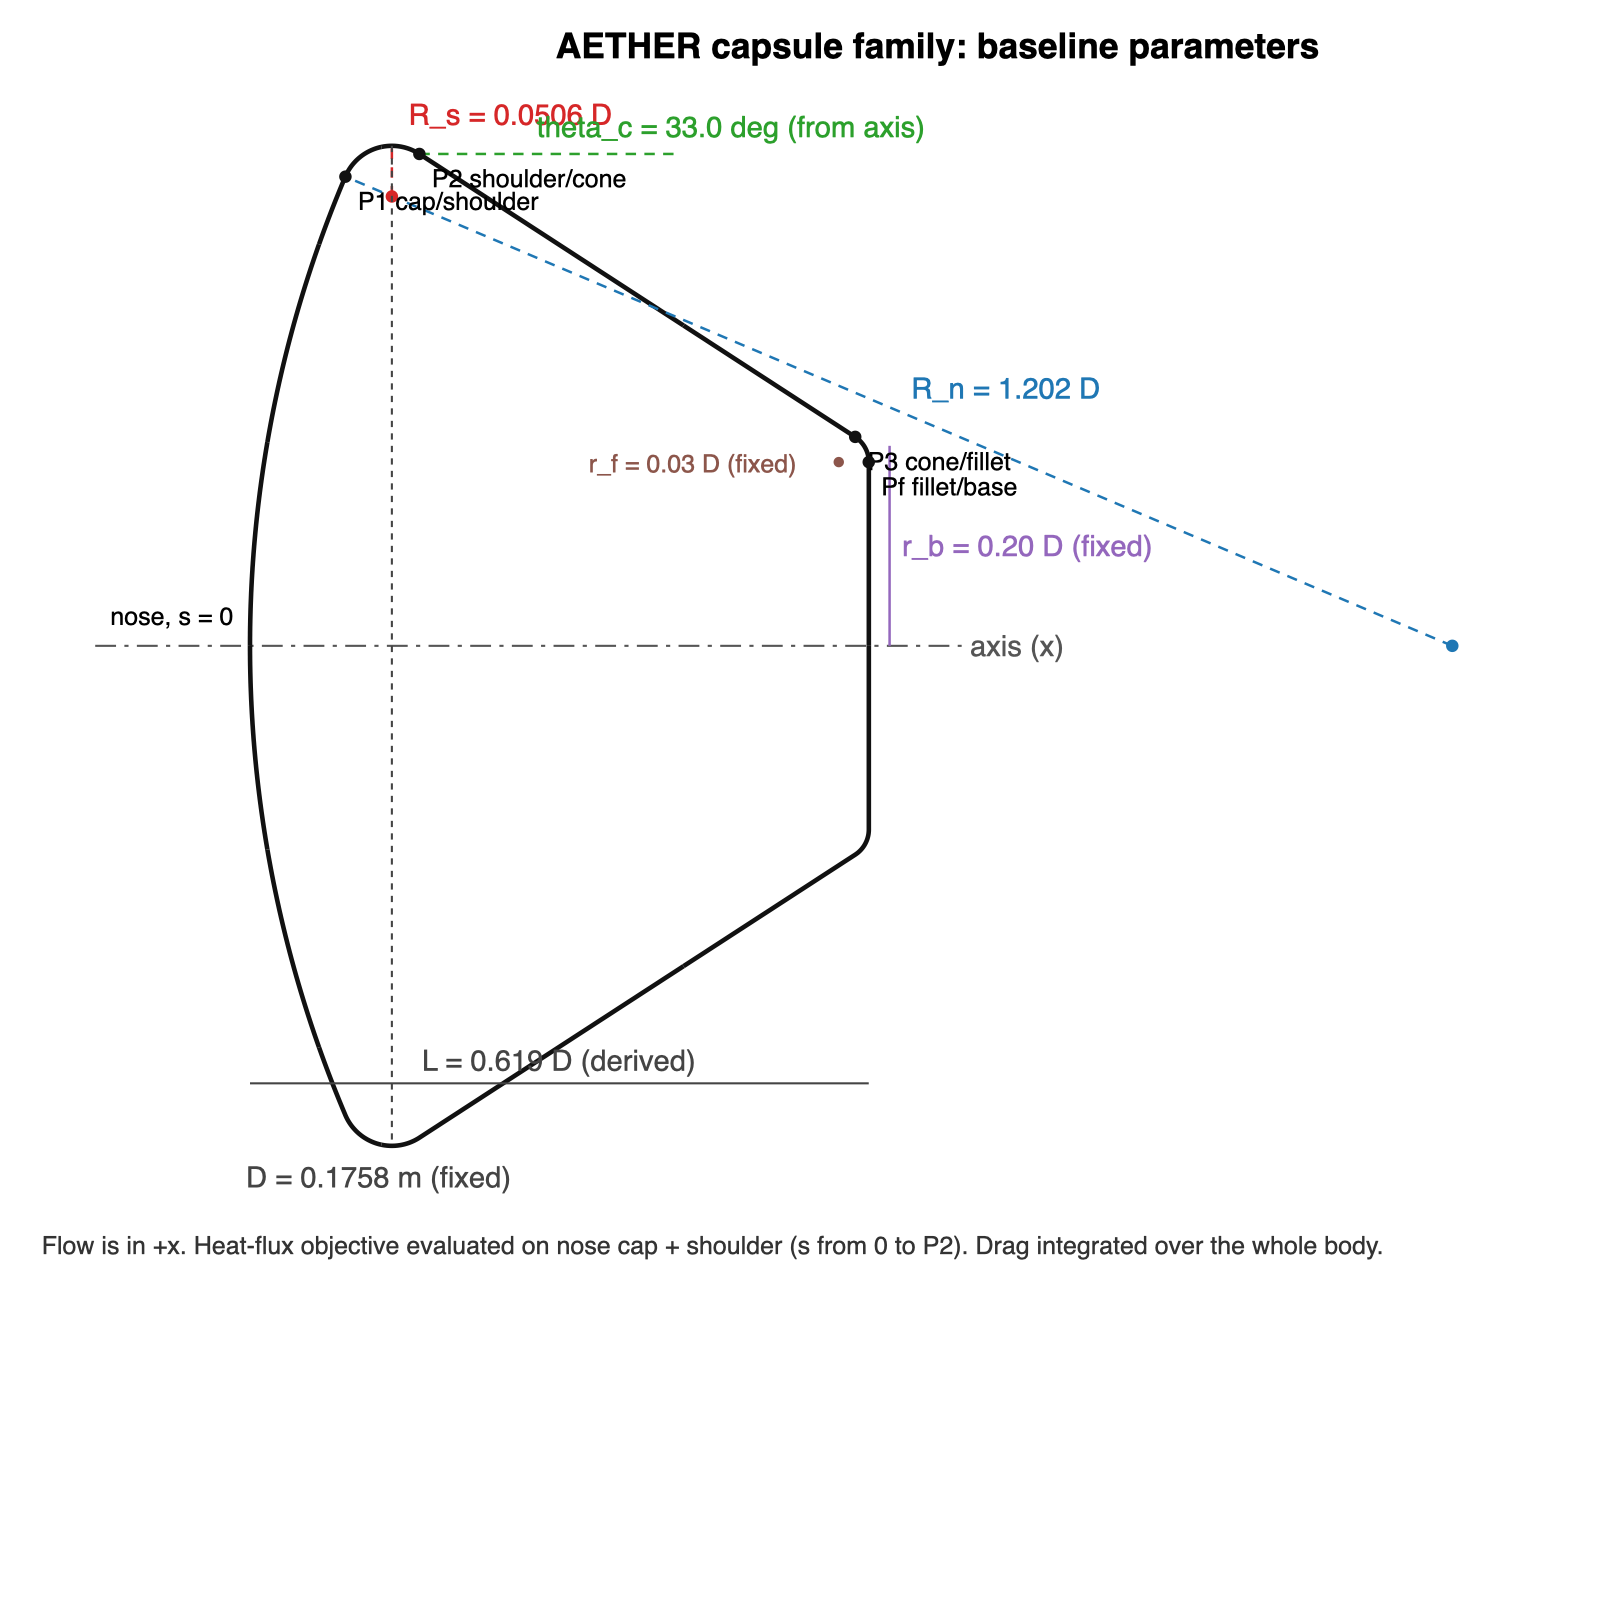
\includegraphics[width=0.70\linewidth]{figure_geometry_baseline.svg.png}
\end{center}
\textbf{One parameter table drives everything:} cap, toroidal shoulder, cone and a fixed closure, joined tangentially; the baseline is the Apollo model itself, so the baseline is also the validation case.
\begin{itemize}
  \item One parameter at a time (nose $0.6$--$1.6\,D$, shoulder $0.03$--$0.18\,D$, cone $25$--$41^\circ$), then five combinations and two deliberately invalid shapes.
  \item Structured meshes from the same table, three nested levels; laminar Navier--Stokes (SU2, axisymmetric); two benchmarks before any design run.
  \item A written rule decides: \emph{lowest peak heating among shapes keeping at least 98\,\% of the baseline drag}; two alternative rules test the choice; shapes differ only beyond the numerical uncertainty.
\end{itemize}
}

%%%%%%%%%%%%%%%%%%%%%%%%%%%%%%%%%%%%%%%%%%%%%%%%%%%%%%%%%%%%%%%% column 2
\column{0.25}

\block{3 \, Building it, and what broke}{
\textbf{Pipeline:} parameter table $\rightarrow$ profile and validity check $\rightarrow$ mesh $\rightarrow$ Roe start-up stage $\rightarrow$ SLAU2 analysis stage $\rightarrow$ post-processing with physical checks $\rightarrow$ \texttt{results.csv}. Every number in the report traces to a case directory with its mesh, configuration, log and history. 59 solver cases, about 45 minutes each on four to six cores.

\vspace{3mm}
\innerblock{Three things the solver did not tell me}{
\begin{itemize}
  \item \textbf{An axis defect.} SU2's axisymmetric source terms produced a heating dip at the stagnation line (second wall node at 154 against a 640--705\,kW/m$^2$ plateau on a sphere test). Fixed by building the solver with a near-axis source-term patch and re-testing.
  \item \textbf{Two steady states.} The first-order scheme has a physical branch and a ``carbuncle'' branch: converged residuals, wrong stagnation pressure. A post-processing check (stagnation pressure against the pitot value, axis heating against the face plateau) now decides for every solution.
  \item \textbf{Converged is not the same as right.} Retries at low CFL passed every monitor and were still slow transients, 8--15\,\% off in heating. The physics said so: shapes with the baseline nose radius must share its plateau heating.
\end{itemize}
}
\vspace{3mm}
\textbf{The fix that worked} was in the mesh, not the schedule: cells elongated along the bow shock (aspect ratio 1.5, and 2 for two stubborn shapes) suppress the instability. Fourteen shapes computed on both mesh families agree to 0.05\,\% in drag and 0.8\,\% in peak heating; the first family stays in the repository as a cross-check.
}

\block{4 \, Evidence that the numbers mean something}{
\begin{center}
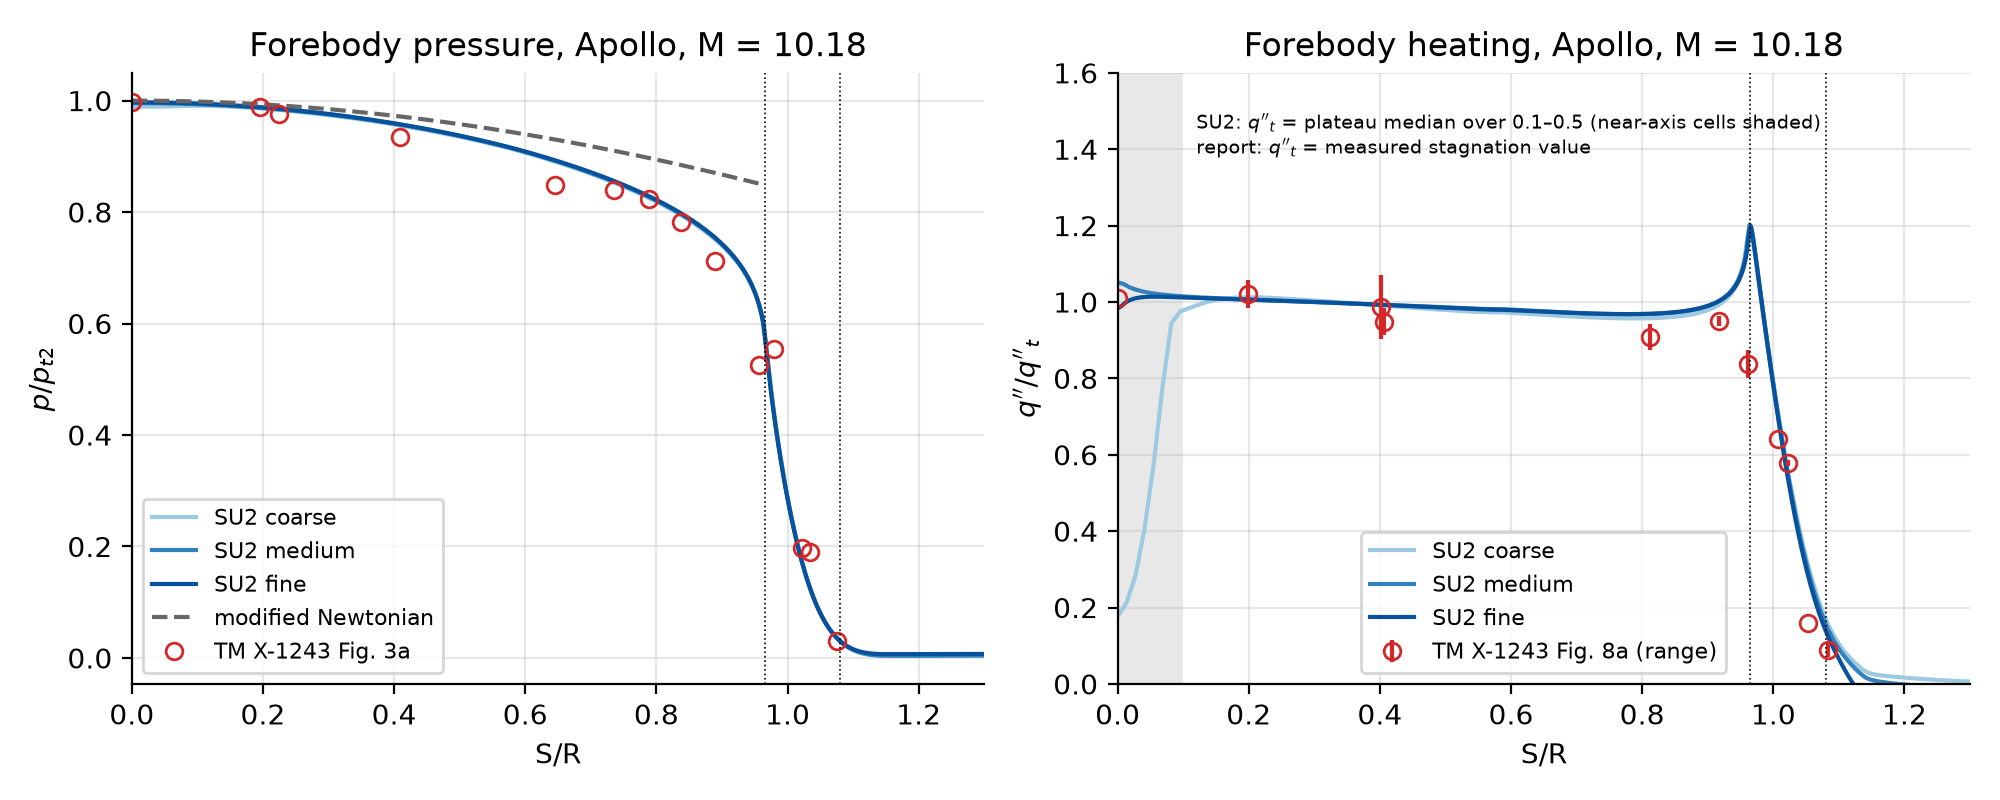
\includegraphics[width=0.92\linewidth]{validation_apollo.png}
\end{center}
\begin{itemize}
  \item \textbf{Apollo, Mach 10.18:} stagnation pressure within 0.5\,\% of pitot; pressure distribution within an rms of 0.05 of the 14 measured stations; face heating flat as measured. SU2 predicts a sharp shoulder peak the thermocouples cannot resolve, so its height is bounded by the mesh study rather than claimed.
  \item \textbf{Wieting cylinder, Mach 8.03:} heating distribution shape within an rms of 0.04--0.06 over 34 stations; absolute level 25\,\% below the shock-tunnel data, the same gap the report notes against theory. Absolute heating is quoted at $\pm 25\,\%$; \emph{differences} between shapes are what the study ranks.
  \item \textbf{Mesh study:} peak heating 112.8 / 110.6 / 109.3\,kW/m$^2$ on coarse / medium / fine, observed order 1.5, GCI 3.1\,\%; drag within 0.15\,\%; far boundary moved out: 0.01\,\% and 0.05\,\%.
\end{itemize}
}

%%%%%%%%%%%%%%%%%%%%%%%%%%%%%%%%%%%%%%%%%%%%%%%%%%%%%%%%%%%%%%%% column 3
\column{0.29}

\block{5 \, Results: the drag--heating trade space}{
\begin{center}
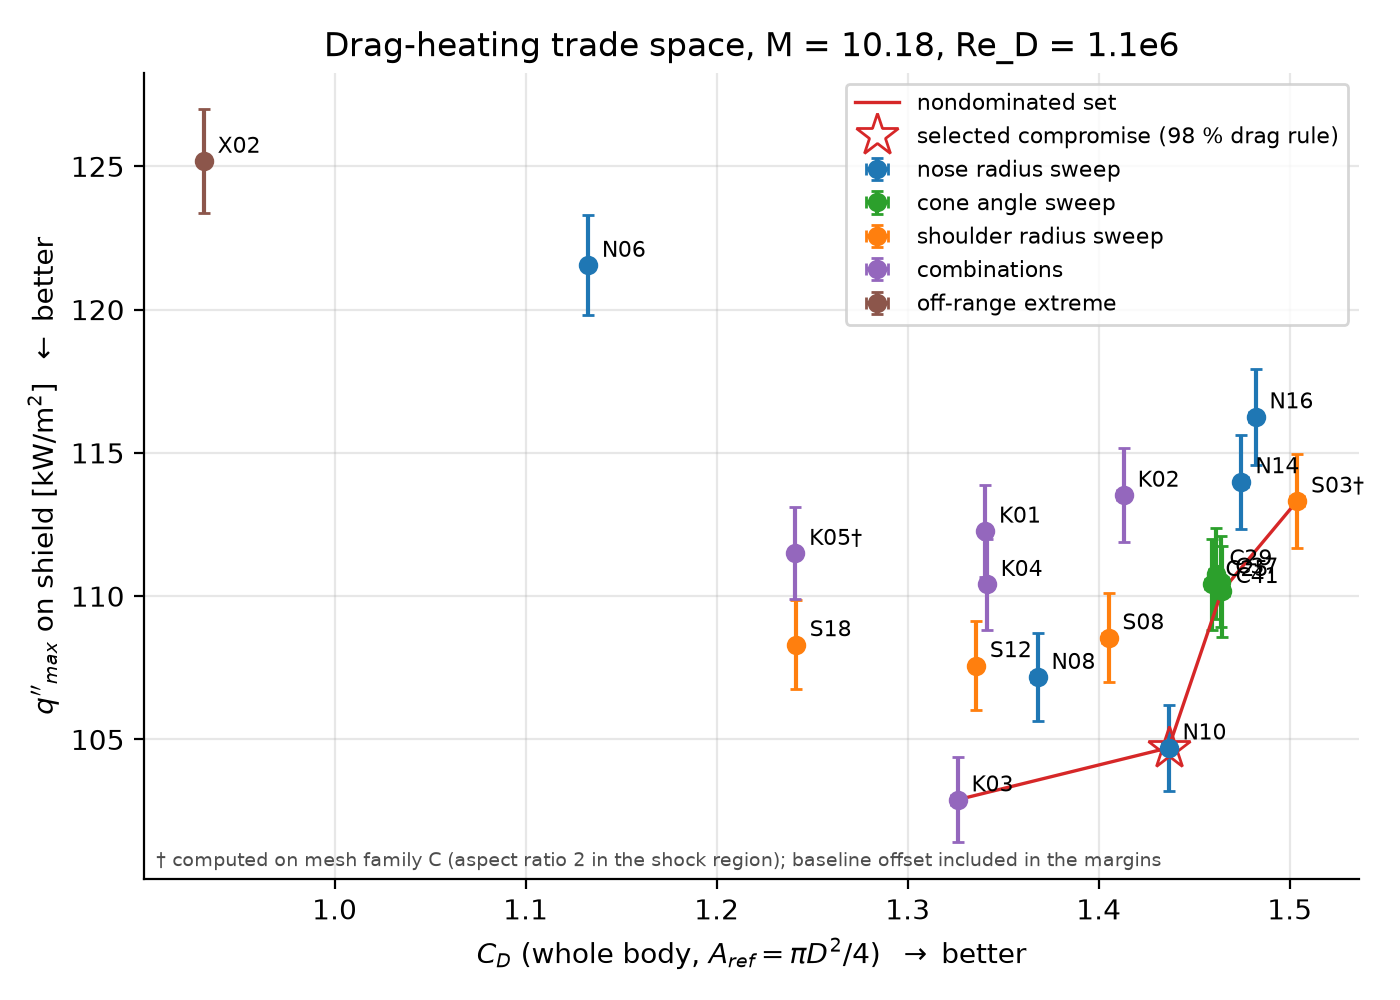
\includegraphics[width=0.80\linewidth]{pareto.png}
\end{center}
\vspace{-2mm}
\begin{itemize}
  \item \textbf{Nondominated set:} S03 (sharp shoulder, $+2.8\,\%$ drag, $+2.5\,\%$ heating), the baseline family, N10 ($R_n/D = 1.0$: $-1.8\,\%$ drag, $-5.3\,\%$ heating), K03 ($R_n/D = 1.0$ with $R_s/D = 0.12$: $-9.3\,\%$, $-6.9\,\%$).
  \item \textbf{The rule picks N10.} The 95\,\% rule picks it too; at 100\,\% of baseline drag nothing beats Apollo beyond the margins.
  \item \textbf{Ranking margins} from fine-mesh re-runs of the finalists: 0.24\,\% in drag, 1.4\,\% in heating. The N10 advantage is four times the margin.
\end{itemize}

\vspace{2mm}
\begin{center}
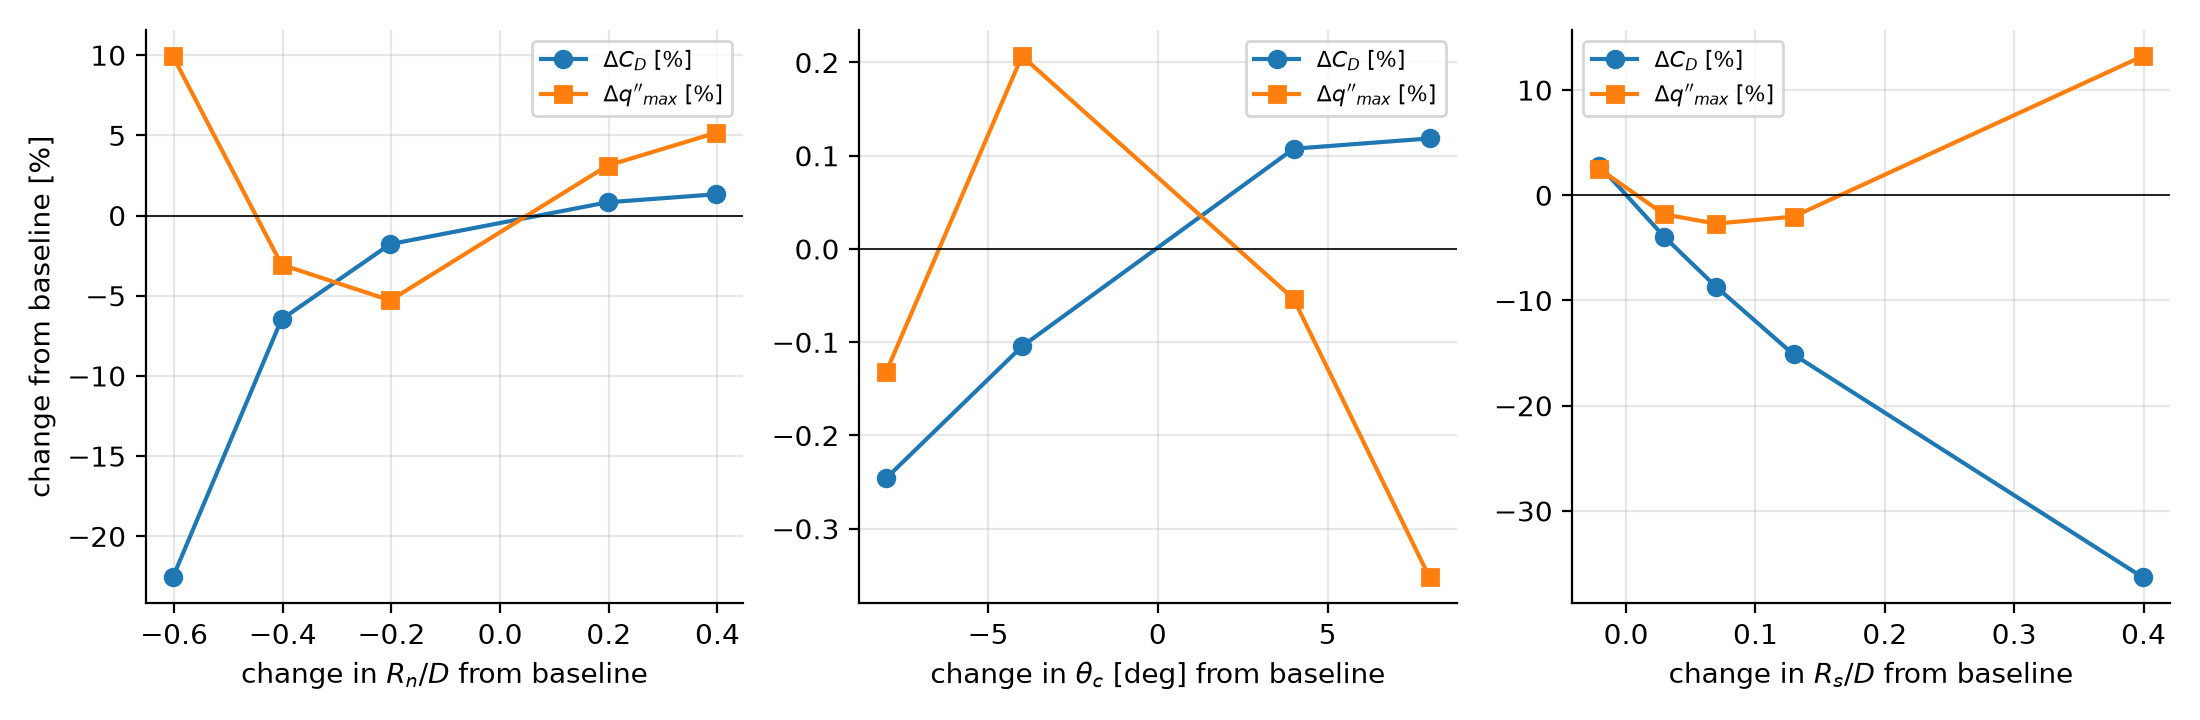
\includegraphics[width=0.90\linewidth]{sensitivities.png}
\end{center}
\vspace{-2mm}
\begin{tabular}{@{}lll@{}}
\toprule
Parameter & Drag & Peak heating \\
\midrule
Nose radius $0.6\to1.6\,D$ & $C_D$ 1.13 $\to$ 1.48 & minimum near $1.0\,D$ \\
Shoulder radius $0.03\to0.18\,D$ & 1.50 $\to$ 1.24 & shallow minimum near $0.12\,D$ \\
Cone angle $25\to41^\circ$ & $<0.4\,\%$ & $<0.4\,\%$ \\
\bottomrule
\end{tabular}
}

\block{6 \, What the flow is doing}{
\begin{center}
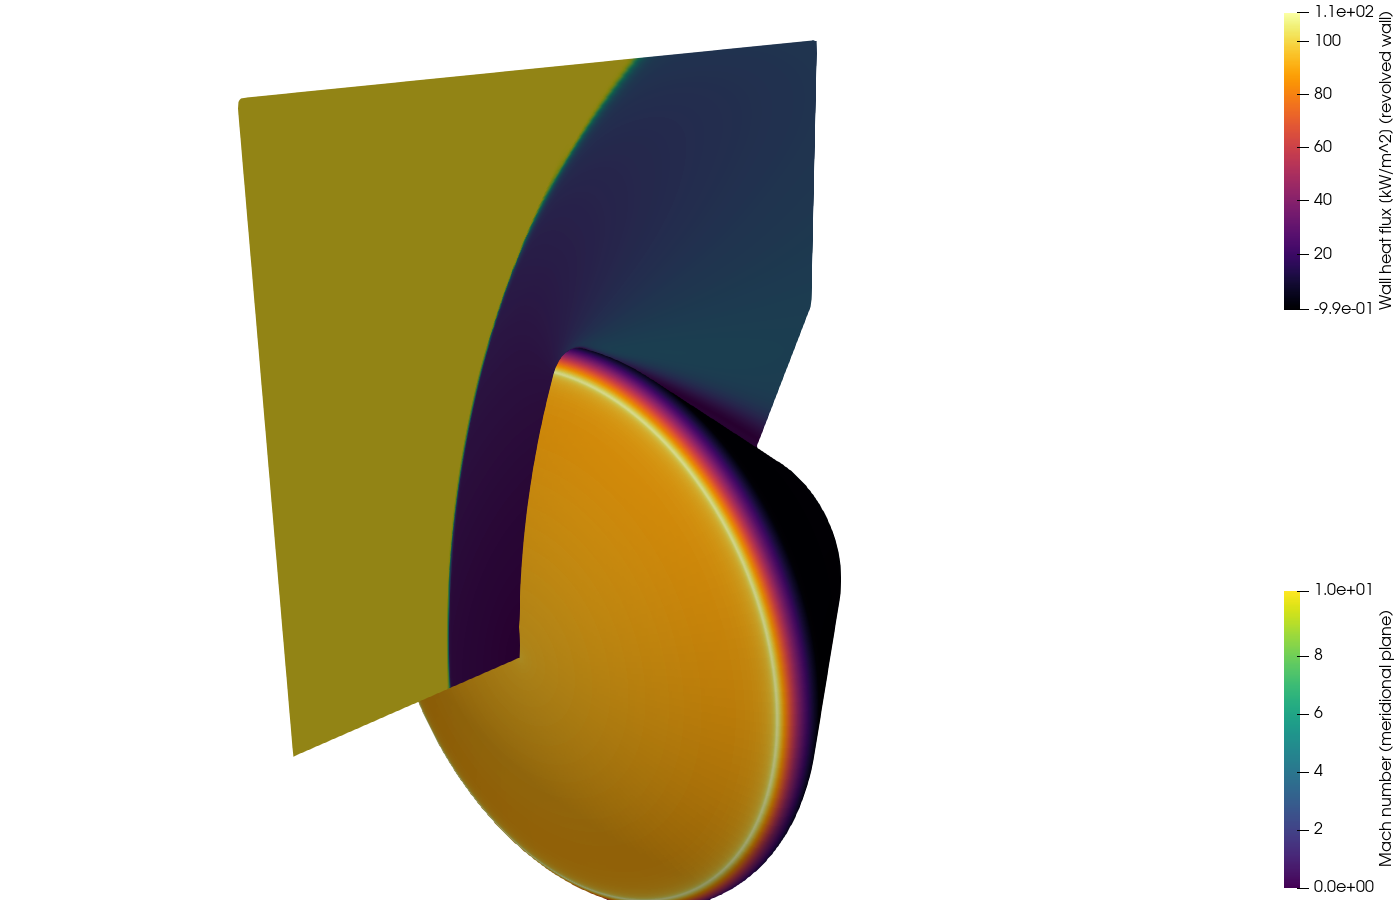
\includegraphics[width=0.40\linewidth]{baseline_Mach_revolved.png}
\end{center}
\vspace{-3mm}
The face sits at nearly the pitot pressure whatever its curvature, so drag is decided by how much of the frontal disc that face covers: large nose radius, small shoulder radius. The peak heating sits at the cap/toroid tangency for every shape with $R_n/D \geq 1$ and grows with the same two parameters. One mechanism drives both objectives, which is why lowering the peak costs drag at a measurable exchange rate: about 2\,\% of drag per 5\,\% of peak heating near the baseline. The revolved view is a visualisation of the axisymmetric solution.
}

%%%%%%%%%%%%%%%%%%%%%%%%%%%%%%%%%%%%%%%%%%%%%%%%%%%%%%%%%%%%%%%% column 4
\column{0.22}

\block{7 \, What I learned}{
\begin{itemize}
  \item \textbf{Write the decision rule before the results exist.} The 98\,\% rule was fixed in the plan; the result was then a finding, not a preference.
  \item \textbf{Validate the tool, then the setup, then the answer.} A planar benchmark isolated the heat-flux prediction from the axisymmetric treatment; that is how the axis defect was found.
  \item \textbf{Residuals are not physics.} Every convergence failure in this study hid behind a satisfied monitor. The checks that caught them were a pitot pressure, a flat face, and a nose-radius scaling law.
  \item \textbf{Uncertainty is a measurement.} The ranking margin was measured (fine-mesh re-runs, a second mesh family), not assumed.
  \item \textbf{Keep the failures.} The abandoned mesh family and every retry are in the repository, tagged, with their numbers; they are the evidence for the method.
\end{itemize}
}

\block{8 \, Honest limits and next steps}{
\begin{itemize}
  \item Perfect gas, laminar, one wind-tunnel condition, cold wall: a ranking of shapes, not a flight heating prediction.
  \item First-order convective fluxes in axisymmetric mode (second order never reached a steady state); the order effect is bounded at 1.3\,\% by the cylinder benchmark.
  \item Base and wake excluded; base force bounded analytically ($\Delta C_D \leq 0.0006$).
  \item Next: the Mach 8 Apollo data as a second condition, a finer shoulder sweep around $R_s/D = 0.08$--$0.12$ combined with $R_n/D = 1.0$, and second order once the solver allows it.
\end{itemize}
}

\block{Reproducibility}{
\small Everything is scripted: \texttt{make all} regenerates meshes, runs, figures and the report. SU2 v8.5.0 built from source with the near-axis patch (\texttt{tools/aether\_su2\_patches.diff}); Python 3.13, Open MPI 5.0.11, ParaView 6.2.0 on an Apple M4. Reference data: NASA TM X-1243 (Bertin, 1966) and NASA TM 100484 (Wieting, 1987). Methods: Celik et al. (2008) for the GCI; Kitamura and Shima (2013) for SLAU2; Fay and Riddell (1958) and Lees (1956) for the heating estimates.
}

\end{columns}
\end{document}
